\section{Material modeling}
This chapter deals with the concept of material modeling based on semi-empirical equations. At first there will be a short overview of the mechanisms of recovery and recrystallization and after that a review of common models describing the evolution of microstructure during hot forming and a way to integrate them into common FEM-software.\par 

\subsection{Recovery and recrystallization}
The flow stress is highly dependent on microstructural softening and hardening mechanism during forming. In addition, these mechanisms are influenced by the temperature, strain rate and strain.\par 

During hot forming, defects are generated within the crystal lattice. According to Gottstein \cite{GOT07} the defects can be distinguished respecting their dimensions. Especially one dimensional defects called dislocations, are the carriers of plastic deformation and therefore crucial for hot working. During hot deformation the density of dislocations rises and hence the resistance of the material to deformation rises too. At a certain point the stored energy in the material is high enough to induce dynamic recovery (DRV) or dynamic recrystallization (DRX). These mechanisms cause softening of the material.\par 

DRV leads to equilibrium between hardening and softening. However DRX leads to a softened material. The effects of DRV and DRX can be well seen in the warm flow curve behavior, see \ref{img:warmflowcurves}.

\begin{figure}[htbp]
 \centering
 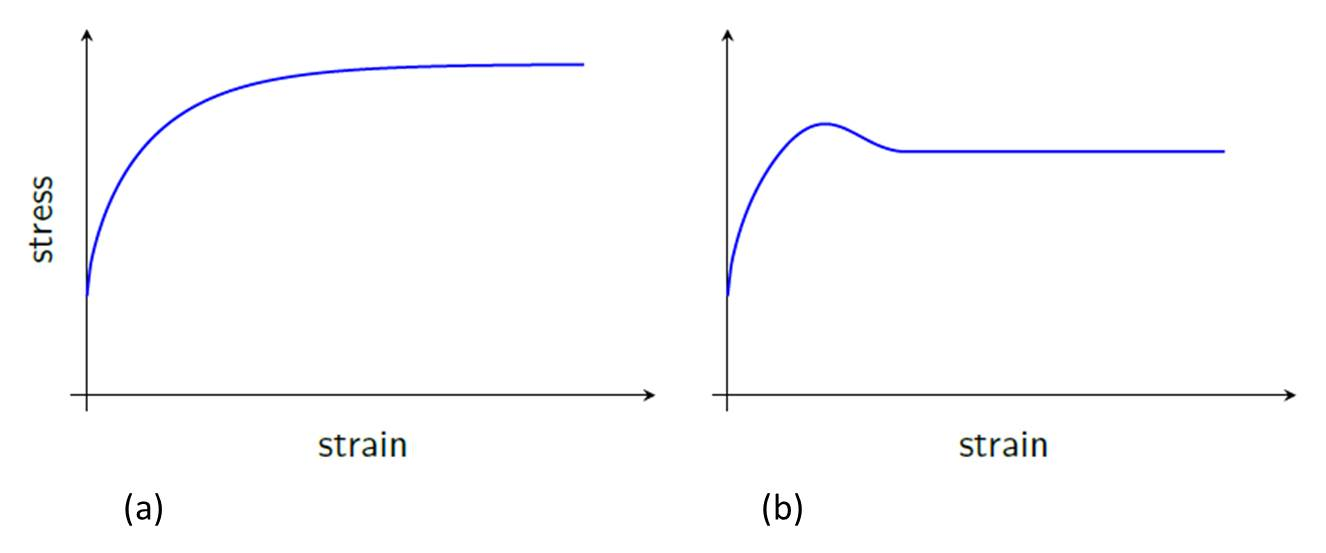
\includegraphics[width=0.8\textwidth]{images/warmflowcurves}
 \caption{Warm flow curves when recovery (a) or recrystallization (b) is predominant \cite{LOH10}}
 \label{img:warmflowcurves}
\end{figure}

The softening effect of DRV and therefore the reduced level of stress with increasing strain is based on the rearrangement and annihilation of dislocations \cite{GOT07}. During DRX new grains are built and grow at spots with low specific energy. Both effects lead to a totally refined microstructure.\par

After hot forming, remaining dislocations can still store a great amount of energy. This energy can be enough to cause static recovery (SRV) or static recrystallization (SRX). These processes take place during heat treatment after warm forming. The softening effects are the same as in DRV or DRX. The driving force drops during SRV and SRX and only when there is enough energy stored, SRV and SRX lead to a fully refined microstructure.\par 

After or parallel to SRV and SRX, grain growth (GG) can take place. The driving force is the reduction of stored energy. During grain growth the nucleated grains grow by using up the old grain structure.\par 

\ref{img:recovandrecrystwarmforming} gives a short summary about the recovery, recrystallization and grain growth mechanisms during warm forming.

\begin{figure}[htbp]
 \centering
 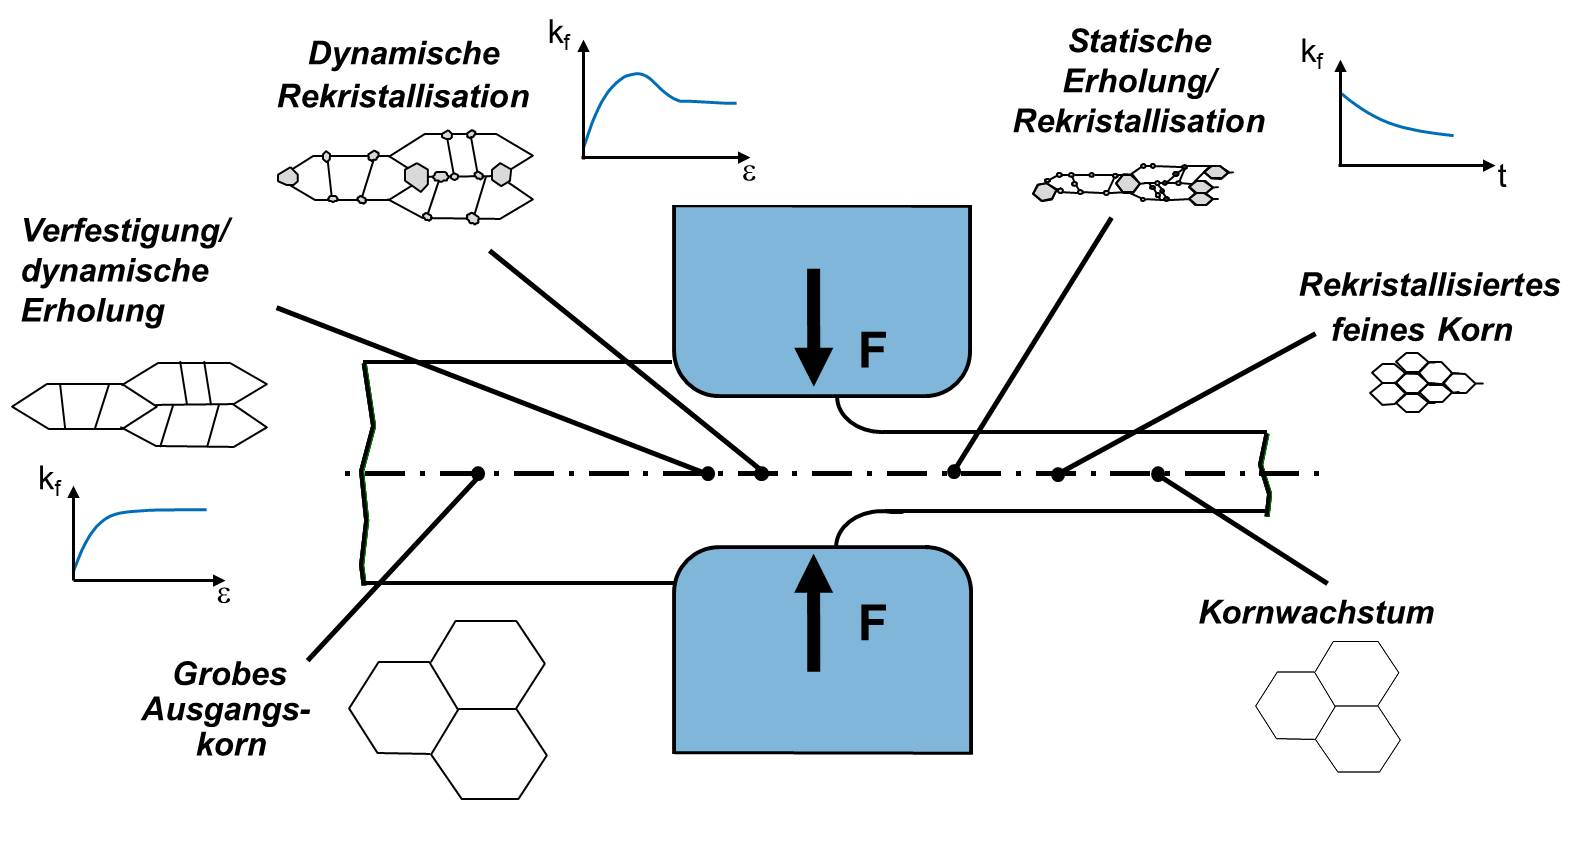
\includegraphics[width=0.8\textwidth]{images/recovandrecrystwarmforming}
 \caption{Recovery and recrystallization mechanisms during warm forming}
 \label{img:recovandrecrystwarmforming}
\end{figure}

The flow curves \ref{img:flowcurves} are essential for the determination of the recrystallization kinetics and the fraction of recrystallized material. Therefore it is the basis for the creation of a microstructure model. At the IBF, flow curves are determined by isothermal compression tests at cylindrical specimens with an height to diameter ratio of 1,5. For the 1.4301 tests have been carried out at temperatures ranging from $900 - 1250 ^{\circ}C$ and strain rates of $0,05 - 100 s^{-1}$ \ref{img:flowcurves}.

\begin{figure}[htbp]
 \centering
 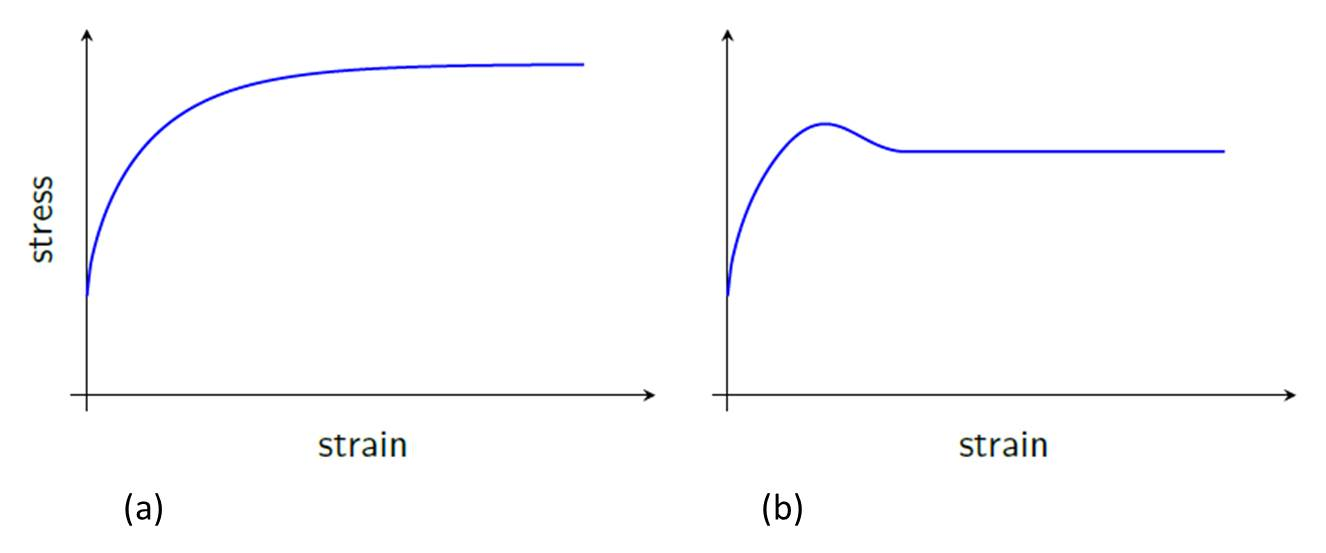
\includegraphics[width=0.8\textwidth]{images/flowcurves}
 \caption{Determined flow curves of 1.4301 (temperature range: 900-1250°C)}
 \label{img:flowcurves}
\end{figure}

For the semi empirical material model given by Deghan Manshadi \cite{DEH08} the special strain values are of great importance. These strain states are seen in \ref{img:stressstrainpoints}. There is the peak strain $\varepsilon_{p}$, the strain of steady state $\varepsilon_{ss}$, and not seen in \ref{img:stressstrainpoints} the critical strain $\varepsilon_{c}$ which is located at 60\%\ of the peak strain. The stresses at these characteristic points are also of importance.

\begin{figure}[htbp]
 \centering
 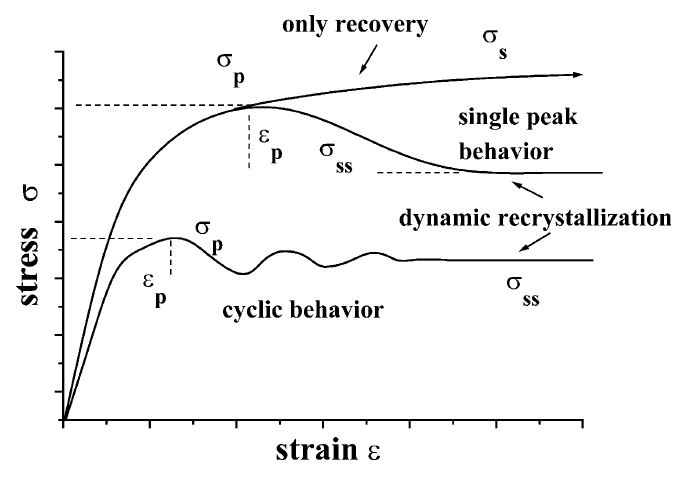
\includegraphics[width=0.8\textwidth]{images/stressstrainpoints}
 \caption{Warm flow curves with characteristic stress and strain points \cite{ELW03}}
 \label{img:stressstrainpoints}
\end{figure}

They can also be calculated by:
\begin{equation}
 \varepsilon_{p} = 3,6\cdot10^{-3}d_{0}^{0}\cdot Z^{0,15}
\end{equation}

\begin{equation}
 \varepsilon_{c} = 0,6\cdot\varepsilon_{p}
\end{equation}

\begin{equation}
 \varepsilon_{ss} = 0,00598\cdot d_{0}^{0}\cdot Z^{0,1536}
\end{equation}

\subsection{Semi emprirical material models}
For the prediction of microstructural evolution semi-empirical models are used for many years. Lohmar and Karhausen gave a detailed overlook over the common models used in warm forming \cite{LOH10}\cite{KAR94}.\par


The JMAK-equation is a way to calculate the fraction of recrystallization RX \ref{img:JMAK} for the different recrystallization mechanisms DRX and SRX. In this work the equation for the calculation of DRX and SRX published by Dehgan Manshadi is used \cite{DEH08}.

\begin{equation}
 X_{DRX} = 1 - exp\left( log\left( 1-0,95\right) \cdot\left( \frac{\varepsilon_{eff}-\varepsilon_{c}}{\varepsilon_{x}}\right) ^{1,3}\right)
\end{equation}

\begin{equation}
 X_{SRX} = 1 - exp\left( log\left( 1-0,5\right) \cdot\left( \frac{t_{SRX}}{t_{50}}\right) ^{1,1}\right)
\end{equation}

Where $t_{50}$ is the time where 50\% recrystallization took place \ref{img:JMAK}:

\begin{equation}
 t_{50} = 8\cdot10^{-9}\varepsilon^{-1,5}\cdot Z^{-0,42}exp\left( \frac{375000}{R\cdot T}\right)
\end{equation}

\begin{figure}[htbp]
 \centering
 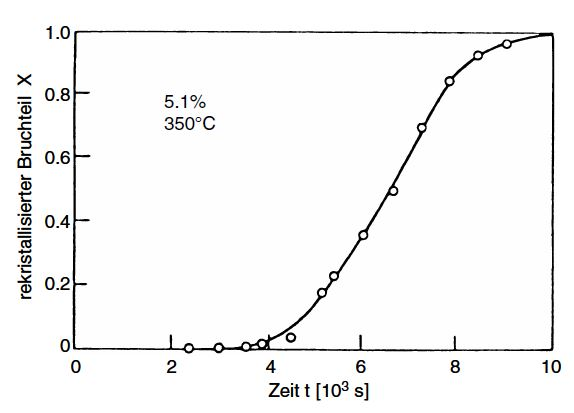
\includegraphics[width=0.8\textwidth]{images/JMAK}
 \caption{Fraction of recrysrallization X}
 \label{img:JMAK}
\end{figure}

A lot of these models relate the stress behavior to the strain rate $\dot{\varepsilon}$ and the Temperature T. A popular way to describe this is given by the Zener-Hollomon parameter Z \cite{ZEN44}:

\begin{equation}
 Z =  \varepsilon\cdot exp\left( \frac{Q}{R\cdot T}\right)
\end{equation}

These equations lead to the determination of the grain size $d_{DRX}$ and $d_{SRX}$ \cite{DEH08}:

\begin{equation}
 d_{DRX} =  5916\cdot Z^{-0,1748}
\end{equation}

\begin{equation}
 d_{SRX} =  4,7\cdot10^{2}\cdot\varphi_{SRX^{-1}}\cdot100^{0,3}\cdot Z^{-0,1}
\end{equation}
